\documentclass[border=8pt]{standalone}
\usepackage{pgfplots}
\pgfplotsset{compat=1.18}
\begin{document}
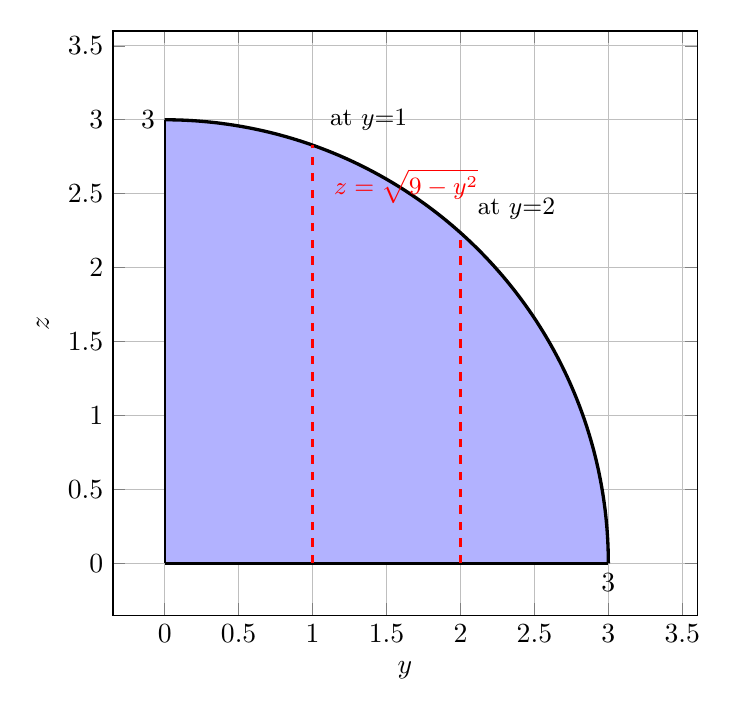
\begin{tikzpicture}
\begin{axis}[
  width=9cm, height=9cm,
  xlabel=$y$, ylabel=$z$,
  xmin=-0.35, xmax=3.6, ymin=-0.35, ymax=3.6,
  trig format plots=deg, grid=major, axis equal,
]
% filled quarter disk
\addplot[fill=blue!30, draw=none, domain=0:90, samples=200] ({3*cos(x)},{3*sin(x)}) \closedcycle;
% cylinder arc
\addplot[very thick, black, domain=0:90, samples=200] ({3*cos(x)},{3*sin(x)});
\addplot[thick, black, domain=0:3, samples=2] ({x},{0});
\addplot[thick, black, domain=0:3, samples=2] ({0},{x});
% constant-y slices : z from 0 to sqrt(9-y^2)
\addplot[thick, dashed, red, domain=0:2.828, samples=2] ({1},{x});
\addplot[thick, dashed, red, domain=0:2.236, samples=2] ({2},{x});
\node[red, font=\small, anchor=west] at (axis cs:1.08,2.55) {$z=\sqrt{9-y^2}$};
\node[anchor=west] at (axis cs:2.05,2.4) {\small at $y{=}2$};
\node[anchor=west] at (axis cs:1.05,3.0) {\small at $y{=}1$};
\node[anchor=north] at (axis cs:3,0) {$3$};
\node[anchor=east] at (axis cs:0,3) {$3$};
\end{axis}
\end{tikzpicture}
\end{document}
